\chapter{\textit{Dataset} do Grupo: Pervisão de burnout em trabalhadores}

\section{Descrição}
\paragraph{}
No cenário acelerado do trabalho moderno, o burnout tem vindo a ganhar destaque como um grande desafio à saúde mental e o bem-estar dos trabalhadores. Esse estado de exaustão emocional e mental, alimentado por pressões constantes, afeta o desempenho dos trabalhadores.

Deste modo, com este \textit{dataset}, o nosso grupo têm como objetivo, numa perspetiva empresarial, determinar o nível de burnout, a partir de outros fatores, para assim tirar o melhor desempenho dos seus funcionários. Para tal, desenvolvemos diversos modelos de machine learning para prever o nível de de burnout dos trabalhadores.

O nosso \textit{dataset} tem as seguintes \textit{features}:
\begin{itemize}
    \item \textbf{Employee ID}: identificador do funcionário (employee)
    \item \textbf{Date of Joining}: Data em que o funcionário começou a trabalhar.
    \item \textbf{Gender}: Género do funcionário
    \item \textbf{Company Type}: Tipo de empresa do funcionário.
    \item \textbf{WFH Setup Available}: Indica se existem sistemas que permitem o trabalho a partir de casa.
    \item \textbf{Designation}: Escalão do funiconário.
    \item \textbf{Resource Allocation}: Número de horas de trabalho por dia.
    \item \textbf{Mental Fatigue Score}: Nível de fadiga mental do funcionário.
    \item \textbf{Burn Rate}: Taxa de burn out de um funcionário.
\end{itemize}

\section{Exploração de dados}
\paragraph{}
A fase de exploração de dados é essencial para compreender o nosso conjunto de dados. Através desta análise conseguimos compreender melhor as cargas de trabalho a que os trabalhadores estão sujeitos e a distribuição de escalões dos mesmos.
Esta fase permitiu ainda identificar padrões e tendências, que ajudaram a tomar decisões sobre as transformações de dados na fase de preparação.

\begin{figure}[H]
    \centering
    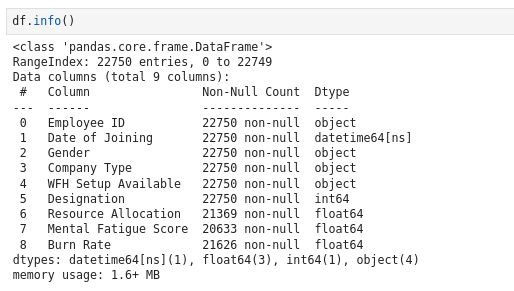
\includegraphics[width=0.8\textwidth]{Imagens/Grupo/info_grupo.png}
    \caption{Método \textit{info()}}
    \label{fig: info_grupo}
\end{figure}

Através do seguinte histograma podemos verificar que a nossa \textit{target} apresenta uma distribuição normal, o que beneficia as tomadas de decisão dos nossos modelos.

\begin{figure}[H]
    \centering
    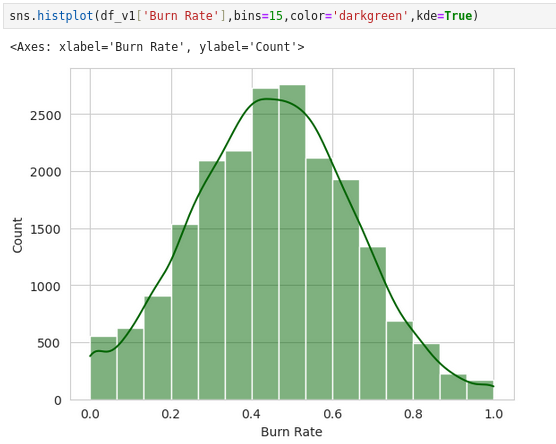
\includegraphics[width=0.7\textwidth]{Imagens/Grupo/histogram_grupo.png}
    \caption{Histograma referente à distribuição dos dados}
    \label{fig: histogram_grupo}
\end{figure}

Para ter uma melhor noção dos dados com que estávamos a trabalhar criamos mais alguns gráficos sendo o mais curioso o seguinte histograma:

\begin{figure}[H]
    \centering
    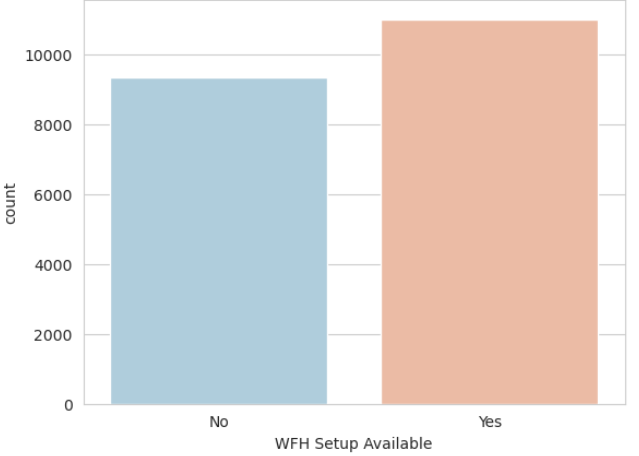
\includegraphics[width=0.7\textwidth]{Imagens/Grupo/local_trabalho.png}
    \caption{Local de trabalho}
    \label{fig: local_trabalho}
\end{figure}

Através deste podemos concluir que a maioria dos trabalhadores trabalha a partir de casa, algo que têm vindo a ser mais recorrente desde a época da pandemia COVID-19.

\begin{figure}[H]
    \centering
    \centerline{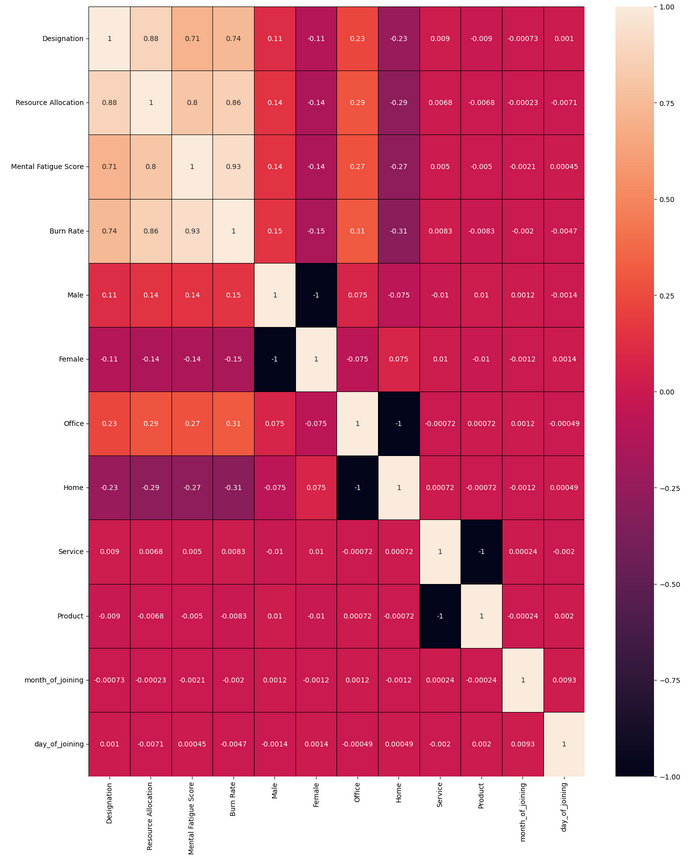
\includegraphics[width=1\textwidth]{Imagens/Grupo/matriz_correlacao_grupo.png}}
    \caption{Matriz de correlação}
    \label{fig: matriz_correlacao_grupo}
\end{figure}

Através do heatmap, podemos constatar algumas correlações entre os dados. Podemos constatar que a nossa \textit{label} tem forte correlação com outras 3 \textit{features} do \textit{dataset}, sendo eles Resource Allocation, Designation e a mais correlacionada, Mental Fatigue Score.

\begin{figure}[H]
    \centering
    \centerline{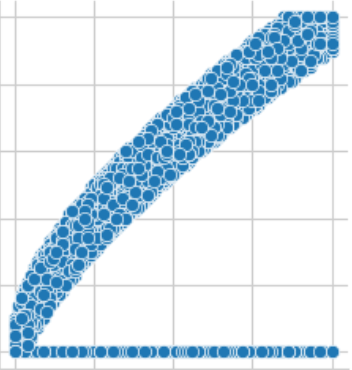
\includegraphics[width=0.5\textwidth]{Imagens/Grupo/seta.png}}
    \caption{Curva de regressão dos dados}
    \label{fig: grafico_azul_grupo}
\end{figure}

Esta última relação é também bem visível no histograma entre ambas no qual podemos tirar ainda a conclusão que embora muito perto, a Mental Fatigue score apresentada nem sempre coincide com o nível de burnout, portanto na sua previsão teremos de utilizar mais \textit{features}.

Foi ainda verificado nesta fase a existência de \textit{missing values} e a não existência de linhas duplicadas.

\begin{figure}[H]
    \centering
    \centerline{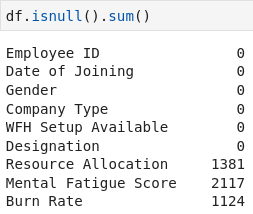
\includegraphics[width=0.5\textwidth]{Imagens/Grupo/missing_values_grupo.png}}
    \caption{\textit{Missing values}}
    \label{fig: missing_values_grupo}
\end{figure}

\section{Preparação de dados}
\paragraph{}
Uma vez que se verificou a existência de \textit{missing values} na fase de exploração, decidimos que as linhas com \textit{missing values} na coluna Burn Rate deviam ser retiradas, uma vez que esta é a nossa \textit{label}. O mesmo tratamento foi efetuado à Resource Allocation.
Para a Mental Fatigue Score não removemos, uma vez que a remoção de todas estas linhas iria equivaler a uma perda de cerca de 15\% dos dados. Por esta razão começamos por preencher os \textit{missing values} com 0, mas rapidamente abandonamos esta opção devido à visualização do gráfico da 'Curva de regressão de dados' anteriormente apresentado. Para um melhor "disfarce" da curva criamos uma função que preenche os \textit{missing values} tendo em conta uma terceira \textit{feature}, sendo decidida a Designation, por ter boa correlação, ficando a curva da seguinte maneira:

\begin{figure}[H]
    \centering
    \centerline{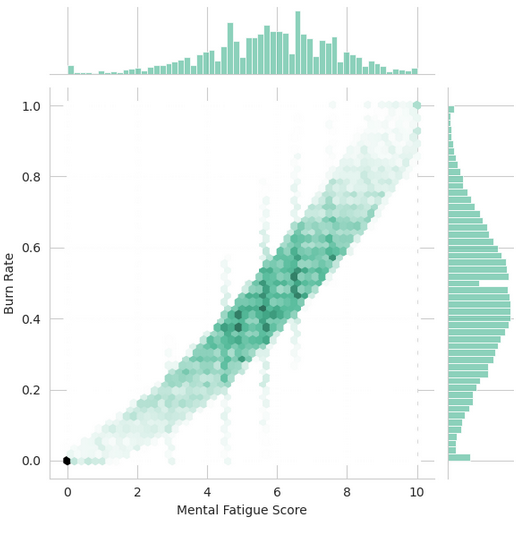
\includegraphics[width=0.7\textwidth]{Imagens/Grupo/curva_grupo.png}}
    \caption{Curva de regressão dos dados}
    \label{fig: curva_grupo}
\end{figure}

Decidimos de seguida retirar a coluna Employee ID, uma vez que é um valor distinto para cada linha e sendo que funciona como um identificador do trabalhador, não trás nenhuma informação relevante para o treino dos nossos modelos.

Para tratar dos dados categóricos foi utilizado one-hot encoding uma vez que os valores destas colunas têm pesos equivalentes e deste modo evitamos uma má influência durante o treino. As colunas que sofreram esta transformação foram: Gender, WFH Setup Available, e Company Type

\begin{minted}[fontsize=\footnotesize, xleftmargin=16pt, breaklines=true, breakanywhere=true]{python}
gender_mapper = {'Male': 0, 'Female': 1}
df_v1['Gender'] = df_v1['Gender'].replace(gender_mapper)
df_v1 = df_v1.join(pd.get_dummies(df_v1['Gender'], prefix='Gender').astype(int))
df_v1.rename(columns={'Gender_0': 'Male', 'Gender_1': 'Female'}, inplace=True)
df_v1.drop(['Gender'], axis=1, inplace=True)
\end{minted}

\begin{minted}[fontsize=\footnotesize, xleftmargin=16pt, breaklines=true, breakanywhere=true]{python}
workplace_mapper = {'No': 0, 'Yes': 1}
df_v1['WFH Setup Available'] = df_v1['WFH Setup Available'].replace(workplace_mapper)
df_v1 = df_v1.join(pd.get_dummies(df_v1['WFH Setup Available'], prefix='WFH Setup Available').astype(int))
df_v1.rename(columns={'WFH Setup Available_0': 'Office', 'WFH Setup Available_1': 'Home'}, inplace=True)
df_v1.drop(['WFH Setup Available'], axis=1, inplace=True)
\end{minted}

\begin{minted}[fontsize=\footnotesize, xleftmargin=16pt, breaklines=true, breakanywhere=true]{python}
company_mapper = {'Service': 0, 'Product': 1}
df_v1['Company Type'] = df_v1['Company Type'].replace(company_mapper)
df_v1 = df_v1.join(pd.get_dummies(df_v1['Company Type'], prefix='Company Type').astype(int))
df_v1.rename(columns={'Company Type_0': 'Service', 'Company Type_1': 'Product'}, inplace=True)
df_v1.drop(['Company Type'], axis=1, inplace=True)
\end{minted}

Foi ainda realizado \textit{feature engineering} na data para verificar se seria obtido mais informação.

Esta fase terminou com a remoção de todas as colunas relativas à data, uma vez que apresentavam uma correlação muito próxima de 0 com todas as outras \textit{features}. Foram ainda retiradas as colunas Product e Service, obtidas do one-hot encoding do Company Type, pelas mesmas razões apresentadas anteriormente.

\section{Modelação}

\subsection{Regressão Linear}
\paragraph{}
Para primeiro modelo, decidimos optar por um modelo simples e recorrentemente utilizado para problemas de regressão, a regressão linear. Tendo como objetivo prever o nível de burnout dos trabalhadores.
\begin{minted}[fontsize=\footnotesize, xleftmargin=16pt, breaklines=true, breakanywhere=true]{python}
lm = LinearRegression()
lm.fit(X_train, y_train)
\end{minted}

Assim sendo, obtivemos os seguintes resultados:
\begin{minted}[fontsize=\footnotesize, xleftmargin=16pt, breaklines=true, breakanywhere=true]{python}
MAE: 0.04872399285439895
MSE: 0.0038600687723920513
RMSE: 0.062129451730979016
\end{minted}

\subsection{Support Vector Regression}
\paragraph{}
Uma vez que utilizamos Support Vector para problemas de classificação nas aulas práticas, tentamos explorar a implementação destes modelos em problemas de regressão utilizando Support Vector Regression.

\begin{minted}[fontsize=\footnotesize, xleftmargin=16pt, breaklines=true, breakanywhere=true]{python}
svr = GridSearchCV(SVR(kernel='rbf'), param_grid={'C': [400,500,600], 'gamma': [1,0.01,0.0001]}, refit=True, verbose=3, scoring='neg_mean_absolute_error')
\end{minted}

Deste modo, obtivemos os seguintes resultados:
\begin{minted}[fontsize=\footnotesize, xleftmargin=16pt, breaklines=true, breakanywhere=true]{python}
MAE: 0.04954229400349311
MSE: 0.0039086508165031226
RMSE: 0.06251920358180454
\end{minted}

\subsection{Rede Neural Artificial}
\paragraph{}
Na implementação das redes neuronais artificiais partimos do modelo utilizado nas aulas práticas, realizando os ajustes necessários como, por exemplo, a dimensão de input.

A arquitetura final obtida pode ser observado de seguida. O modelo utilizado tem 4 camadas. A primeira possui então 7 neurónios relativos ao número de \textit{features}, as seguintes têm respetivamente 16,9 e 1.

\begin{minted}[fontsize=\footnotesize, xleftmargin=16pt, breaklines=true, breakanywhere=true]{python}
def build_model(activation='relu', learning_rate=0.01):
    model = Sequential()
    model.add(Dense(16, input_dim=7, activation=activation))
    model.add(Dense(9, activation=activation))
    model.add(Dense(1, activation=activation))
    
    model.compile(loss='mae', optimizer=tf.optimizers.Adam(learning_rate), metrics=['mae','mse'])
    return model
\end{minted}

\begin{minted}[fontsize=\footnotesize, xleftmargin=16pt, breaklines=true, breakanywhere=true]{python}
optimizer = ['SGD','RMSprop','Adagrad']
activation = ['sigmoid','relu']
param_grid = dict(optimizer=optimizer)
\end{minted}

\begin{minted}[fontsize=\footnotesize, xleftmargin=16pt, breaklines=true, breakanywhere=true]{python}
kf = KFold(n_splits=5, shuffle=True, random_state=2021)
\end{minted}

\begin{minted}[fontsize=\footnotesize, xleftmargin=16pt, breaklines=true, breakanywhere=true]{python}
model = KerasRegressor(model=build_model, batch_size=100, validation_split=0.2, epochs=80)
\end{minted}

\begin{minted}[fontsize=\footnotesize, xleftmargin=16pt, breaklines=true, breakanywhere=true]{python}
grid_search = GridSearchCV(estimator=model, param_grid=param_grid, cv=kf, scoring='neg_mean_absolute_error', refit='True', verbose=1)
\end{minted}

Para verificar se a arquitetura das redes neuronais não estavam a entrar em situação de overfitting, seguimos o exemplo da aula e criamos o seguinte gráfico:

\begin{figure}[H]
    \centering
    \centerline{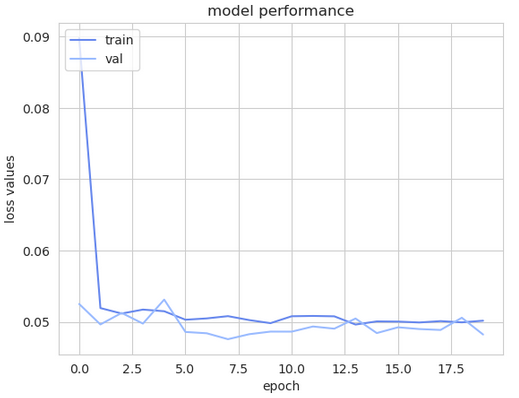
\includegraphics[width=0.7\textwidth]{Imagens/Grupo/ANN.png}}
    \label{fig: ANN}
\end{figure}

Após a sua análise consideramos que estamos na presença de um bom modelo.

Assim sendo, obtivemos os seguintes resultados:
\begin{minted}[fontsize=\footnotesize, xleftmargin=16pt, breaklines=true, breakanywhere=true]{python}
MAE: 0.048217227288524116
MSE: 0.0037480777355242247
RMSE: 0.06122154633398461
\end{minted}

\subsection{Gradient Boosting}
\paragraph{}
Criados os 3 últimos modelos decidimos partir para a implementação de um modelo sugerido pela professora durante o \textit{checkpoint}, o Gradient Boosting.

\begin{minted}[fontsize=\footnotesize, xleftmargin=16pt, breaklines=true, breakanywhere=true]{python}
param_boost = {'learning_rate': [0.01,0.02,0.03], 'subsample': [0.1, 0.2, 0.4], 'n_estimators': [128,256,512], 'max_depth': [4,8,12]}
\end{minted}

\begin{minted}[fontsize=\footnotesize, xleftmargin=16pt, breaklines=true, breakanywhere=true]{python}
estimator_boost = GradientBoostingRegressor()
grid_boost = GridSearchCV(estimator_boost, param_boost, refit=True, verbose=0)
\end{minted}

\begin{minted}[fontsize=\footnotesize, xleftmargin=16pt, breaklines=true, breakanywhere=true]{python}
{'learning_rate': 0.03, 'max_depth': 4, 'n_estimators': 512, 'subsample': 0.4}
\end{minted}

Finalmente, obtivemos os seguintes resultados para este último modelo:
\begin{minted}[fontsize=\footnotesize, xleftmargin=16pt, breaklines=true, breakanywhere=true]{python}
MAE: 0.045546670468378576
MSE: 0.00329982576622636
RMSE: 0.057444109935017355
\end{minted}

\section{Avaliação}
\paragraph{}
Após implementados os três modelos, realizamos então uma comparação entre os resultados obtidos.
Para obter uma perceção mais visual entre os MAE obtidos em cada um, criamos o seguinte gráfico de barras:

\begin{figure}[H]
    \centering
    \centerline{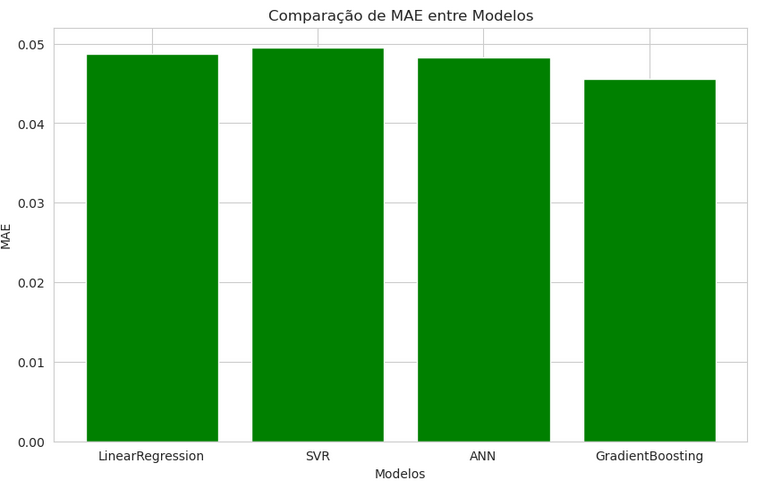
\includegraphics[width=1\textwidth]{Imagens/Grupo/MAE.png}}
    \label{fig: MAE}
\end{figure}

Como é possível observar, o modelo que apresentou melhor resultados foi o Gradient Boosting, no entanto, a diferença entre este resultado não é muito significativa quando comparado com os outros modelos.

Por outro lado, outro fator que podemos ter em conta é o tempo que cada um destes demorou para treinar e executar as previsões. Neste aspeto, a regressão linear ganha uma certa vantagem por ser mais simples e demorar cerca de 2 segundos para executar enquanto que os outros três modelos demoram 3 minutos ou mais.

Tendo estes dois fatores em conta, consideramos então que na necessidade de efetuar uma previsão o mais acertada possível, sem limites a nível de tempo, o modelo a ser utilizado deve ser o Gradient Boosting sendo o que apresentou melhores resultados.

Se as previsões tiverem de ser efetuadas o mais rápido possível e/ou os recursos disponíveis não forem os melhores possíveis, para estes casos, o grupo considera que a utilização de Regressão Linear é uma alternativa válida pois é um algoritmo mais leve e que obteve bons resultados, como podemos observar.
